\chapter{Week 1 - Introduction}
\textit{4-09-2017 \\
Johanna Höffken \\} 

\section{What is sustainable development according to Brundtland?}
According to Brundtland sustainable development is development that meets the needs of the present without compromising the ability of future generations to meet their own needs. \\
\\
This is one of the most common definition in the field of sustainability by Brundtland in 1987. The definition can be seen as a challenge to the conventional model of socio-economic development rooted in the modernization theory. Brundtland's formulation represents the mainstream thinking about the environment-development relationship. 

\section{What are the seven environmental critiques?}
\begin{enumerate}
\item \textsc{Limited understanding of progress}: progress as seen as the extent at which nature is made useful. Domination over nature;
\item \textsc{Priority to economic growth}: environmental deterioration is an inevitable side effect;
\item \textsc{Human welfare equals consumption}: welfare is measured by individual income that is spent on purchasing goods. 
\item \textsc{Poor understanding of social stability};
\item \textsc{Western domination over developing countries}: Western development based on resources from the global south. The process of overexploitation leading to underdevelopment and culture of dependence;
\item \textsc{Western style of development cannot be replicated globally}: there are just not enough resources;
\item \textsc{Failure to recognize limits to economic growth}: capacity of the Earth, there are limits.
\end{enumerate}

\section{What is the Conventional Development Theory?}
In 1960, the American economic historian Rostow suggested that countries passed through five stages of economic development:
\begin{enumerate}
\item \textsc{Traditional society} with subsistence, barter and agriculture;
\item \textsc{Transitional stage} with specialization, surpluses and infrastructure;
\item \textsc{Take off} with industrialization, growing investment, regional growth and political change;
\item \textsc{Drive to maturity} with diversification, innovation, less reliance on imports and investments;
\item \textsc{High mass consumption} with consumer oriented durable goods, service sector becomes dominant. 
\end{enumerate}
The Conventional Development Theory sees the progression in development as linear in which countries catch up and converge with the Western style of development. 

\begin{figure}[ht]
\begin{center}
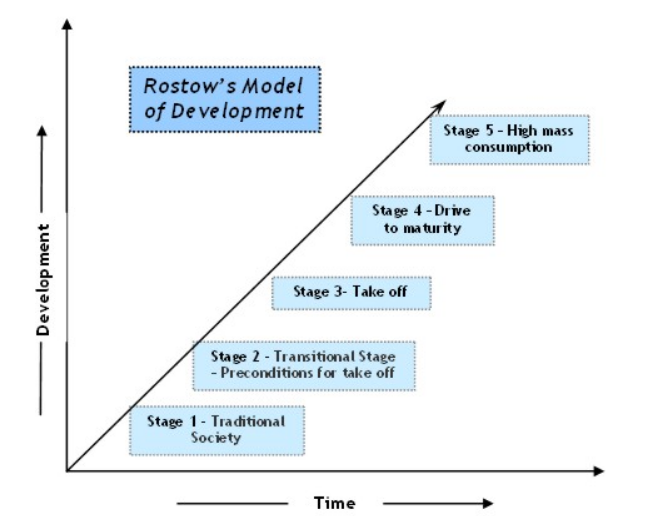
\includegraphics[scale=0.9]{Rostow}
\end{center}
\end{figure}

\section{How is sustainable development seen as a holistic approach?}
Sustainable development is a 	holistic approach because it denotes what is socially just, economically efficient and within the boundaries of the nature. It therefore combines society, economy and ecology. The model accounts of interdependencies and causal links. 

\section{How is sustainable development seen as a dynamic approach?}
Sustainable development is dynamic because the desirable characteristics and meanings change and will change over time. Besides this, they will also change across space (e.g. differences between regions in the world). Sustainable Development recognizes diversity and plurality with evolving meanings across social, political, cultural and historical context. 

\section{On what moral principles is sustainable development based? (According to the normative approach)}
\begin{itemize}
\item \textsc{Common but differentiated responsibilities}: every country contributes to the crisis in different ways. Also, every country have different capabilities to take action. 
\item \textsc{Intra- and inter- generational equity}: justice within and between generations. Equity between rich and poor, North and South. 
\item \textsc{Participation}: involvement of those outside formal governmental bodies. Sustainable Development is subjective (people disagree about ideals and values).
\item \textsc{Gender equality}.
\end{itemize}

\section{What are the two philosophical interpretations of sustainable development?}
Sustainable Development has multiple interpretations and philosophical underpinnings:
\begin{itemize}
\item \textsc{Anthropocentric}: wealth of nature seen only in relation to its mankind; manipulation of nature; pragmatic approach (left).
\item \textsc{Ecocentric}: nature has intrinsic value, human-nature partnership; principled approach (right).
\end{itemize}

\begin{figure}[ht]
\begin{center}
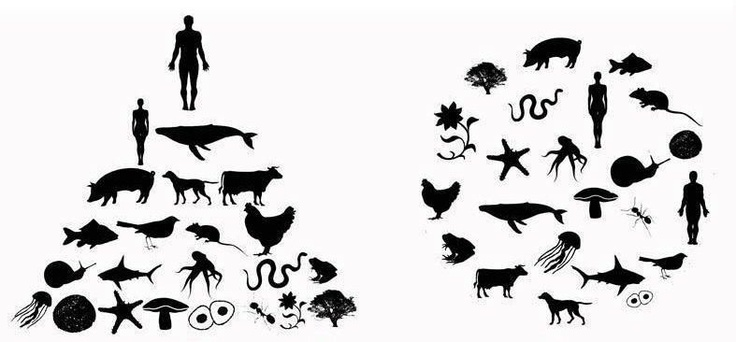
\includegraphics[scale=0.5]{SDviews}
\end{center}
\end{figure}

\clearpage

\section{What is Baker's ladder of sustainable development?}
\begin{itemize}
\item \textsc{Pollution control:} environmental protection is important, but should not put limits on development or constrain human freedom to innovate. Technology can solve any environmental problem. Provides Environmental Kuznets Curve as evidence.

\begin{figure}[ht]
\begin{center}
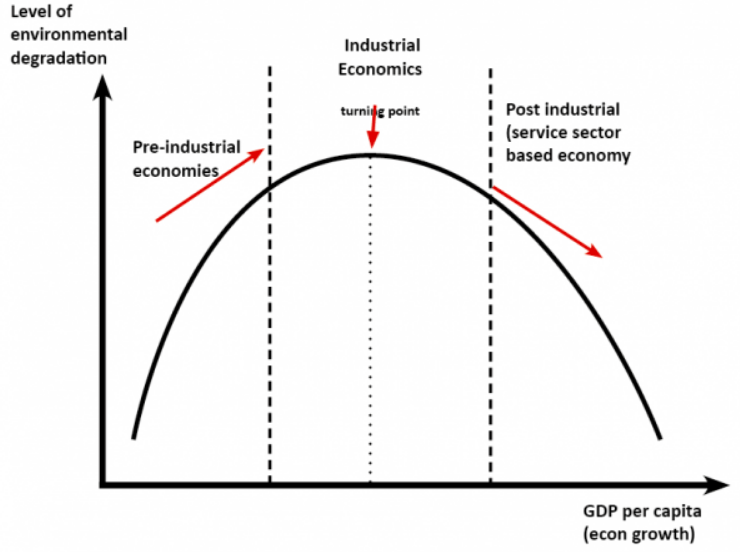
\includegraphics[scale=0.75]{Kuznet}
\end{center}
\end{figure}

\item \textsc{Weak sustainable development:} economic approach to sustainable development. Pricing is important for natural resources: best way to preserve them. Strong belief in technological substitutes. Ecological modernization: economy benefits from environment. Policies promoting economic growth. 
\item \textsc{Strong sustainable development:} environment a pre-condition for development, not the other way around. Limits to technological fixes. Shift from growth to non-material aspects of development. Attention to development in other world regions. From quantitative GDP to qualitative HDI and quality of life. 
\item \textsc{Ideal sustainable development:} attributes equal value to all life forms. Non-interference with nature. Rejects managerial interference in nature. Laborintensive technologies. Bottom up community structures 
\end{itemize}

\section{What is Cleantech?}
Cleantech is a shortened form of "clean technologies", a term used to describe an investment philosophy used by investors seeking to profit from environmentally friendly companies. Cleantech firms seek to increase performance, productivity and efficiency by minimizing negative effects on the environment.

\clearpage